%\documentclass[a4paper, 11pt, addpoints]{exam}
%%\documentclass[a4paper, 11pt, addpoints, answers]{exam}  % Desconmente esta linha, para ver as respostas, e comente a de cima
%\usepackage{listaufersa}
%\usepackage{listings} % Mostrar código-fonte
%\usepackage[brazil]{babel}
%\usepackage{multicol}
%\usepackage{booktabs}
%\usepackage{hyperref}
%
%\setlength{\columnsep}{25pt}
%\lstdefinestyle{js}{
%    basicstyle=\ttfamily,
%    breaklines=true,
%    breakatwhitespace=true,
%    tabsize=1,
%    resetmargins=true,
%    xleftmargin=0pt,
%    frame=none
%}
%
%
%
%
%%%%%%%%%%%%%%%%%%%%%%%%%%%%%%%%%%%%%%%%%%%%%%%%%%
%
%\pointpoints{Ponto}{Pontos}
%
%\begin{document}
%
%
%%%%%%%%%% Informações sobre o curso %%%%%%%%%%%%%
%
%
%\nomeProfessor{Rodrigo Toledo Teixeira Câmara}
%\nomeCurso{Bacharelado em Ciências e Tecnologias}
%\nomeDisciplina{Cálculo Numérico}
%\semestre{5}   % Deixe em branco se for para mais de um semestre (recuperação)
%\dataDaProva{2016.2}
%\tipoAvaliacao{lista da aula 06}
%
%\info
%\vspace{-0.5 cm}
%
%
%%%%%%%%%%%%%%%%%%%%%%%%%%%%%%%%%%%%%%%%%%%%%%%%%%
%
%
%
%\begin{questions}
%%\begin{multicols}{2}
\section{Método da bissecção}

\begin{ex}\label{primeirasitbi}
Utilizando o \emph{GeoGebra}, estime, em cada função, um intervalo que possua uma raiz. Em seguida, com auxílio de uma calculadora, faça as duas primeiras iterações do método da bissecção. Ao final de cada iteração, calcule 
\begin{itemize}
\item a diferença absoluta entre duas candidatas a solução, 
\item a diferença relativa entre duas candidatas a solução, 
\item o comprimento do intervalo e 
\item a diferença absoluta entre $f(\overline{x})$ e $0.$
\end{itemize}
\begin{enumerate}
\item $f(x)=x+e^x$,
\item $f(x)=\sin(x)-x^2+1$,
\item $f(x)=x^3-\sin(x)$,
\item $f(x)=3x-\cos(x)+1$,
\item $f(x)=\ln(x)-\sin(x)$.
\end{enumerate}
\begin{sol}
\begin{enumerate}
\item A escolha do intervalo que possui raiz é livre. Para esta solução, irei supor que o intervalo escolhido foi $[-2,0]$. Pelo algoritmo da bissecção, as duas primeiras iterações geram os intervalos $[-1,0]$ e $[-1,-0.5]$. Com o intervalo escolhido, a candidata inicial $x_0$ é $-1$. As duas primeiras candidatas a solução calculadas são $x_1=-0.5$ e $x_2=-0.75$. A diferença absoluta entre essas candidatas são $d_1=0.5$ e $d_2=0.25$.  
\end{enumerate}
\end{sol}
\end{ex}

\begin{ex}
Estime quantas iterações são necessárias para achar a raiz de cada uma das funções da questão \ref{primeirasitbi} pelo método da bissecção, considerando a precisão $\epsilon$, $\epsilon=0.001$. 
\end{ex}


\begin{ex}
Encontre as raízes das funções da questão \ref{primeirasitbi} com precisão $\epsilon$, com $\epsilon=0.001$, utilizando o critério de parada que você julgar mais apropriado.
\end{ex}

\section{Métodos do Ponto Fixo}
\begin{ex}\label{ex1mpf}
Considere a função dada $f$ dada por $$f(x)=x^6+4x^2-20.$$
\begin{enumerate}
\item Trace o gráfico desta função no \emph{GeoGebra}  e estime a menor raiz positiva. 
\item Utilizando a forma geral $$\varphi(x)=x+A(x)f(x),$$ com $A(\xi)\neq 0$, construa três funções iterativas $\varphi$.
\item Verifique se alguma destas funções iterativas converge para a menor raiz positiva de $f$.
\end{enumerate}
\end{ex}
\section{Método de Newton-Raphson}
\begin{ex} Seja $f$ a função da questão \ref{ex1mpf}.
\begin{enumerate}
\item Determine a função $\varphi$ conforme proposta pelo método de Newton-Raphson.
\item Calcule as duas primeiras iterações deste método.
\end{enumerate}
\end{ex}

\begin{ex}\label{newton}
Considere a função $f$ dada por
$$ g(x) = x^8 + 6x^2 - 4x + 0.6655.$$ 
\begin{enumerate}
\item Trace o gráfico desta função no \emph{GeoGebra}  e estime a menor raiz positiva.
\item Determine, utilizando o método de Newton-Raphson e precisão $\epsilon=0.01$, a raiz $\overline{x}$ desta função com o seguinte critério de parada:
\begin{enumerate}
\item Diferença absoluta entre duas candidatas a solução.
\item Diferença absoluta entre $f(\overline{x})$ e $0$.
\end{enumerate}
Comente cada um dos resultados.
\end{enumerate}
\end{ex}

\section{Método da secante}
\begin{ex}
Calcule as duas primeiras iterações do método da secante das funções dadas abaixo. Esboce os gráficos das funções no \emph{GeoGebra} para estimar as duas aproximações iniciais da menor raiz positiva.
\begin{enumerate}
\item $f(x)=x^2-10.$
\item $g(x)=x\sin(x).$
\item $h(x)=(x-2)^2-\ln(x).$
\end{enumerate}
\end{ex}


\section{Problemas}

\begin{ex}
Os métodos de busca de raízes de função podem ser utilizados para encontrar \emph{soluções de equações}. Sugira uma forma para \emph{resolver} equações. Utilizando esta forma, encontre um número $x$ tal que $$e^x=x^2.$$
\end{ex}

\begin{ex}
Descreva uma forma de encontrar (e encontre) a raiz quadrada de 7 com treze algarismos significativos. Depois, encontre a raiz cúbica de 10 com treze algarismos significativos. Dica: a raiz quadrada de $a$ é encontrada ao se calcular a raiz da função $f(x)=x^2-a$.
\end{ex}




\begin{ex}\label{prob.coluna}
Uma das tarefas mais importantes de um engenheiro civil é calcular a carga máxima que uma estrutura pode suportar. Uma previsão errada pode fazer a construção se romper, trazendo prejuízos financeiros, risco à integridade física de trabalhadores e atraso no cumprimento de prazos.

Para uma coluna presa pela base, carregada excentricamente com tensão $\sigma$, utiliza-se o seguinte modelo matemático para calcular a carga axial máxima suportada:
\begin{equation}
f(x)=\frac{x}{A}-\frac{\sigma}{1+\frac{e c}{r^2}\sec{\left(\frac{L}{2r}\sqrt{\frac{x}{E A}}\right)}},
\label{eq.cam}
\end{equation}
onde $L$ é o comprimento da coluna em metros, $c$ e $r$ são constantes positivas referentes às propriedades geométricas das colunas, $e$ é uma constante que determina a excentricidade da carga e $E$ é o módulo de Young, uma constante que depende da elasticidade do material utilizado. A função $\sec$ é a função trigonométrica ``secante''.

A carga axial máxima suportada, $P_{max}$, dada em \emph{newtons}, é a \emph{menor raiz positiva} da função dada pela equação \ref{eq.cam}.

Considere uma estrutura construída com os parâmetros dados na tabela \ref{tab.parametros_coluna}.

% Please add the following required packages to your document preamble:
% \usepackage{booktabs}
\begin{table}[hb]
\centering
\caption{Valores das constantes usadas na equação \ref{eq.cam}.}
\label{tab.parametros_coluna}
\begin{tabular}{@{}ll@{}}
\toprule
Constante & Valor (em unidades do Sistema Internacional) \\ \midrule
$A$       & $1$                                            \\
$c$       & $1$                                            \\
$r$       & $1$                                            \\
$\sigma$  & $4*10^4$                                     \\
$E$       & $3*10^7$                                     \\
$e$       & $0.3$                                          \\
$L$       & $50$                                           \\ \bottomrule
\end{tabular}
\end{table}

Determine a carga axial máxima suportada por esta construção.
\end{ex}

\begin{ex}\label{prob.matfin}
 A equação que relaciona a taxa de juros $i$ com o valor à vista $PV$, o valor fixo $PMT$ de cada parcela e a quantidade $n$ de parcelas  é
 $$PMT=PV \frac{i(1+i)^n}{(1+i)^n-1}.$$


Supondo que uma geladeira é vendida à vista por $R\$1500,00$ e que a loja permite o pagamento em doze parcelas iguais de $R\$150,00$, calcule a taxa de juros deste financiamento.
\end{ex}
\begin{ex}\label{prob.vigas}\emph{(Problema das vigas)}
Duas vigas de madeira de 20 e 30 metros se apóiam nas paredes de um galpão como mostra a figura \ref{fig.vigas}. Se o ponto em que se cruzam está a 8 metros do solo, qual é a largura deste galpão?
\begin{figure}
\center
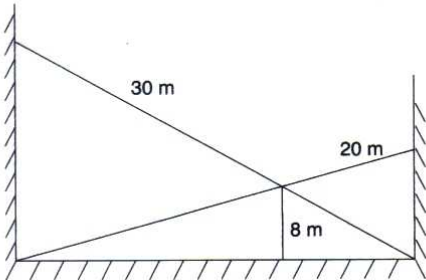
\includegraphics[width=0.6\linewidth]{vigas.png}
\caption{Vigas de 30 e 20 metros, apoiadas nas paredes de um galpão.}\label{fig.vigas}
\end{figure}

\end{ex}